\documentclass{jsarticle}

%----------------------------------
% 文章の中に 画像を入れるための設定
%----------------------------------
\usepackage[dvipdfmx]{graphicx}

%----------------------------------
% 自分の作る文章の題
%----------------------------------
\title{上腕三頭筋の働きと鍛え方}

%---------------------------------- 
% 文書を作った日
%----------------------------------
\date{\today}

%----------------------------------
% 自分の名前を入れる
%----------------------------------
\author{山 根 千 佳}

%---------------------------------------------------
% 文書のスタイルを決める設定
%---------------------------------------------------
\usepackage[height=26cm,width=16cm]{geometry}

%-----------------------------------
% 以上で下準備は終わりです.
% ここから表示される文章を作成していきます.
%-----------------------------------
\begin{document}

%----------------------------------------
% 文章に上に、上記で記述したタイトル、
% 文書を作成した日にち, 著者の名前を書き込みます.
%
% (注)\maketitle をはずせば, タイトル, 日にち,著者名は文書に挿入されません.
%----------------------------------------

\maketitle

%--------------------------------------------
% 主な内容はここから
%--------------------------------------------

\section{目的}
本レポートは、腕の曲げ伸ばし運動における上腕二頭筋と上腕三頭筋の役割を推測することを目的とした。具体的には、腕の曲げ伸ばし運動が遅い場合と速い場合の2パターンにおいて、筋電位の変化と腕の各関節の位置変化を同時に計測する。これにより、上腕二頭筋と上腕三頭筋において、腕の曲げ伸ばし以外の機能を探すことを目的とした。

\section{実験方法}
被験者は、膝をついた状態で座り、腕を床と水平に繰り返し曲げ伸ばしした。
計測は、腕の伸縮をゆっくり行った場合と、早く行った場合との2パターンについて行った。
本実験における被験者は1人であった。
                                                                                                                                                                                                                                                                                                                                                                                                                                                                                                                                                                                                                                                                                                                                                                                                                                                                                                                                                                                                                                                                                                                                                                                                                                                                                                                                                                                                                                                                                                                                                                                                                                                                                                                                                                                                                                                                                                                                                                                                                                                                                                                                                   
\subsection{計測実験}
実験には、MotionCapture(ライブラリ社 MoveTR)と筋電計(ロジカルプロダクト社)を用いた。
MotionCaptureでは、被験者の運動の様子を真上からカメラで撮影し、肩、肘、手首の3点を追跡することで、各関節の位置座標の変化を200 fpsで計測した。

筋電計は上腕二頭筋および上腕三頭筋に貼付し、サンプリング周波数1000 Hzで各筋電データを取得した。

\subsection{取得データの解析}
筋電データには、1〜40 Hzのバンドパスフィルタ(signal.buttord 関数)をかけた。また、バンドパスフィルタをかけることにより生じる時間のずれを、filtfit 関数により自動補正した。
このデータをもとに、時刻$t$における筋肉の活動度$a(t)$を、
$$a(t) = \frac{1}{\Delta T} \int_{t-\frac{\Delta T}{2}}^{t+\frac{\Delta T}{2}} |E(t)|dt $$
として求めた。つまり、ある時刻$t$における筋肉の活動度を、その前後$\Delta T = 10$ [ms]のデータ値を平均して求めた。
これにより、生データにおける波形の不規則さが残らないようにした。$\Delta T$の値は、筋収縮の変化に追いつけるよう留意した。

\clearpage
\section{結果}

\begin{figure}[h]
	\begin{center} %センタリングする
		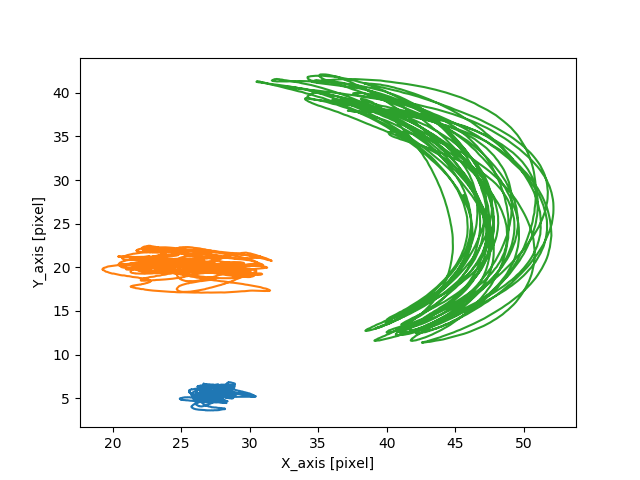
\includegraphics[width=10cm]{graph_image/slow_kidou.png}
		\caption{腕の3関節の軌道} %タイトルをつける
		\label{fig:kidou} %ラベルをつけ図の参照を可能にする
	\end{center}
\end{figure}
図\ref{fig:kidou}はゆっくりと腕の曲げ伸ばし運動を行った場合の、各関節の位置変化を示す。
水色、オレンジ、黄緑はそれぞれ、肩、肘、手首の軌道を示している。
この図から、今回の実験では、手首における変化が3関節の中でもっと大きい。また、手首において、Y軸方向への位置変化がX軸方向に比べて大きいことがわかる。そこで、本レポートでは、筋電データと、Y軸方向への手首の動きの相関に注目した。

\begin{figure}[!h]
	\begin{center}
		(a)
		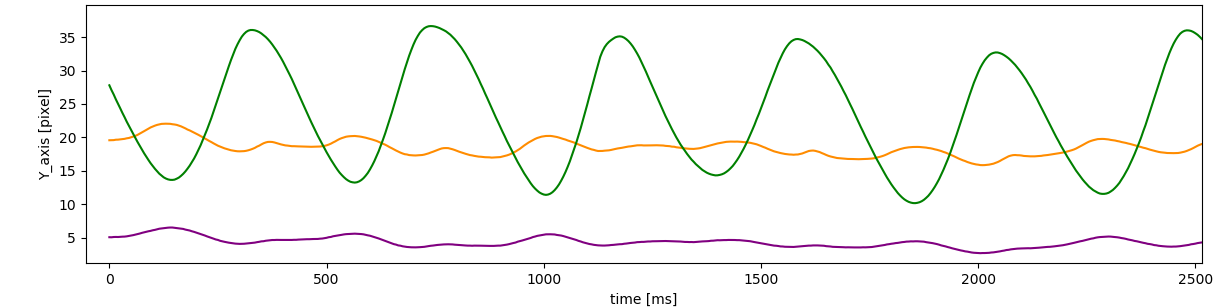
\includegraphics[width=17cm]{graph_image/fast_position.png}
		\label{fig:fast_position}
		(b)
		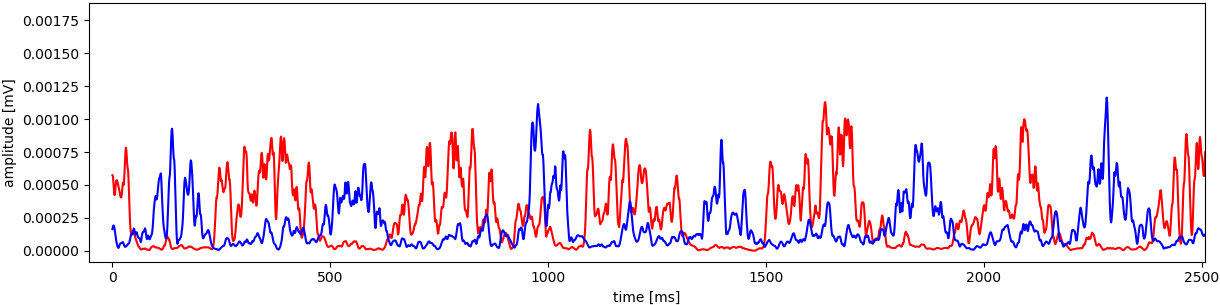
\includegraphics[width=17cm]{graph_image/fast_EMG.png}
		\caption{腕の曲げ伸ばし速度が遅い時の筋電データ。(a)は各関節の位置変化、(b)は筋電データである。}
		\label{fig:fast_EMG}
	\end{center}
\end{figure}
\clearpage

\begin{figure}[!h]
	\begin{center}
		(a)
		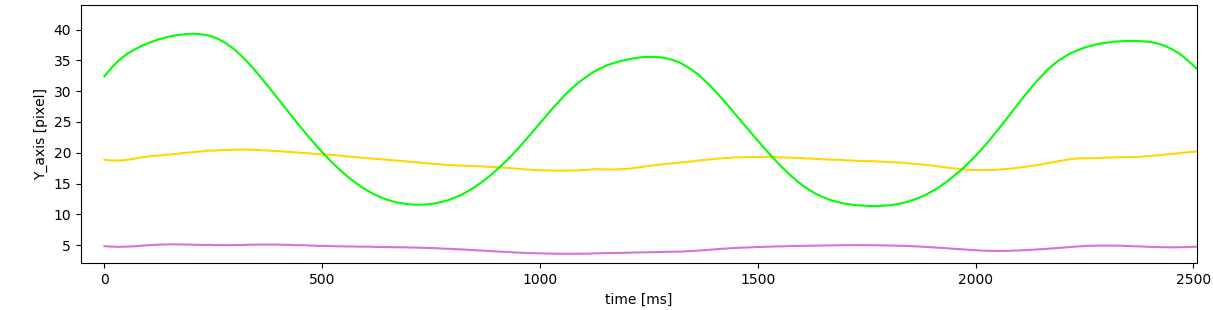
\includegraphics[width=17cm]{graph_image/slow_position.png}
		\label{fig:slow_position}
		(b)
		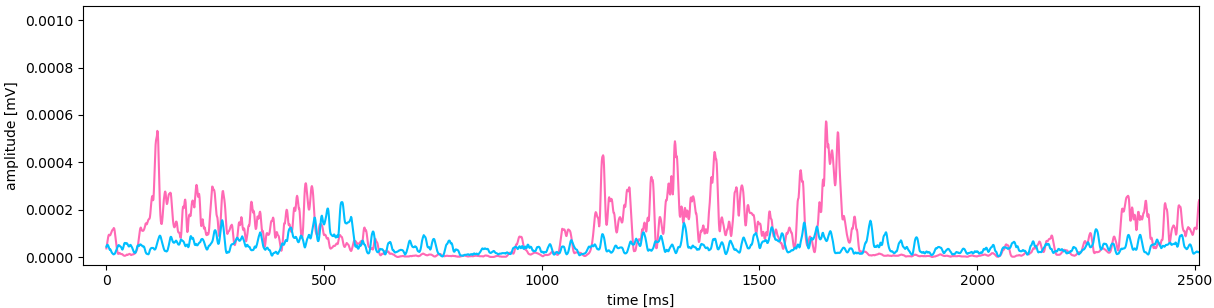
\includegraphics[width=17cm]{graph_image/slow_EMG.png}
		\caption{腕の曲げ伸ばし速度が遅い時の筋電データ。(a)は各関節の位置変化、(b)は筋電データである。}
		\label{fig:slow_EMG}
	\end{center}
\end{figure}


図\ref{fig:fast_position} (a)は、腕の曲げ伸ばし運動を速く行った場合の、各関節のY軸方向への時間変化である。紫、オレンジ、緑はそれぞれ肩、肘、手首の軌道を表す。
図\ref{fig:fast_EMG} (b)は、赤が上腕二頭筋、青が上腕三頭筋の筋電データであり、縦軸は活動電位、横軸は時間である。
これら2つの図において、上腕二頭筋の筋活動は、Y軸方向の手首の動きと逆位相になっていた。つまり、腕が曲がるほど、上腕二頭筋における多くの筋繊維で活動電位が発生した。また、上腕三頭筋の筋電位は、腕を伸ばすタイミングで上昇した。これらの結果から、腕が曲がる際に上腕二頭筋が収縮し、腕が伸びる際に上腕三頭筋が収縮することがわかる。

図\ref{fig:slow_position} (a)は、上段が腕の曲げ伸ばし運動を遅く行った場合のY軸方向の位置変化である。薄紫、黄色、黄緑はそれぞれ肩、肘、手首の位置変化を示す。
図\ref{fig:slow_EMG} (b)は、ピンクが上腕二頭筋、水色が上腕三頭筋の筋電データである。
遅い腕の曲げ伸ばしでは、上腕二頭筋の筋活動は、腕を曲げるタイミングで大きくなっており、速い場合と同様であった。しかし、腕の伸縮が遅い場合では、上腕三頭筋の筋活動は腕を伸ばすタイミングで一概に大きくなっておらず、小さな振幅のまま変化があまり見られなかった。

これらの結果から、上腕二頭筋は腕の伸縮速度に関わらず、腕が曲がる際に収縮していることがわかる。一方、上腕三頭筋は、腕の伸縮が速いときは、腕が伸びる際に筋収縮が起こるが、腕の伸縮が遅い場合には、腕を伸ばす運動と筋収縮に相関があると言い切れない結果となった。このことから、上腕三頭筋には腕の伸展以外の役割があることが示唆される。

\section{考察}

上腕二頭筋は、腕を曲げる働きがあり、上腕三頭筋は腕を伸ばす働きがある\cite{reference1}。今回の結果では、腕の伸縮の速度を変化させると、上腕三頭筋の筋電位に特徴的な違いが見られた。腕の伸縮が速い場合、上腕三頭筋の筋電位は、腕を伸ばすタイミングで上昇した。また腕の伸縮が遅い場合、上腕三頭筋の筋電位は0に近かったが、完全に0となることはほぼなく、小さな振幅を維持していた。
私はこのことから、腕の伸縮が遅い場合の筋電位には、腕を伸ばすための活動電位に加えて、肩から腕までの部分を地面と水平に保持する筋力を発生させるための活動電位が含まれていると考えた。つまり、上腕三頭筋には、肘を伸ばす役割の他に、肩から肘までの位置を固定・維持する役割があるのではないかと考えた。

そもそも筋肉は、関節をまたいで骨に結合している。関節トルクは、筋収縮に伴って2つ以上の骨が引っ張られることで生成される。ここで、上腕三頭筋は、肩関節と肘関節をまたいだ2関節筋である\cite{reference2}。
このことから、腕を上げる高さに応じて、上腕三頭筋の収縮の程度が変化する(腕を高く上げるほど上腕三頭筋が強く収縮する)と予想できる。よって、腕をある程度の高さまで持ち上げて固定するという運動は、上腕三頭筋の収縮によるものであるという考察の妥当性が高まった。

このことを踏まえて、腕の伸縮が速いときの筋電位について見ると、腕を曲げている際にも、振幅が見られ、この振幅が腕の位置固定に伴う活動電位であると推測できる。また、腕の伸縮が速い場合の、上腕三頭筋の筋電位の振幅は、腕の伸縮が遅いときの振幅に比べて大きかった。これは、腕を速く動かすことにより、腕の位置を地面と水平方向に固定することがより難しくなり、多くの筋力が必要となるためであると考えることができる。

これらのことから、上腕三頭筋を鍛えるためには、腕の曲げ伸ばし運動に加えて、肩から腕の位置固定を物理的に難しくするトレーニング(例えば、肩から腕までの部位に重いリングのようなものをかけた状態で腕を素早く曲げ伸ばしするなど)が有効なのではないかと考えられる。

\begin{thebibliography}{9}
	\bibitem{reference1} 「3D 踊る肉単」 河合良訓,原島広至 pp.xiv
	\bibitem{reference2} 「3D 踊る肉単」 河合良訓,原島広至 pp.38
\end{thebibliography}
%--------------------------------------------
% 文章これまで.
%--------------------------------------------
\end{document}
